\documentclass[a4paper]{article}


\usepackage[utf8]{inputenc}
%\usepackage[T1]{fontenc}
\usepackage[francais]{babel}
\usepackage[left=4.2cm,right=4.2cm,top=3cm,bottom=3cm]{geometry}
\usepackage{graphicx,amsmath,amsthm, amssymb,amsfonts,nicefrac}
\usepackage[svgnames,hyperref]{xcolor}
\usepackage[backref=page, colorlinks, linktocpage, citecolor = blue, linkcolor = blue, urlcolor=blue]{hyperref}
\usepackage{enumitem}
\usepackage{caption}
\usepackage{subcaption}
\usepackage{animate}
\usepackage{zref}

\usepackage{listings}
\usepackage{algorithm}
\usepackage{algorithmic}
\usepackage{color}

\usepackage{titlesec}
\setcounter{secnumdepth}{4}

\definecolor{dkgreen}{rgb}{0,0.6,0}
\definecolor{gray}{rgb}{0.5,0.5,0.5}
\definecolor{mauve}{rgb}{0.58,0,0.82}

\lstset{frame=tb,
  language=Python,
  aboveskip=3mm,
  belowskip=3mm,
  showstringspaces=false,
  columns=flexible,
  basicstyle={\small\ttfamily},
  numbers=none,
  numberstyle=\tiny\color{gray},
  keywordstyle=\color{blue},
  commentstyle=\color{dkgreen},
  stringstyle=\color{mauve},
  breaklines=true,
  breakatwhitespace=true,
  tabsize=3
}

%%%%%% Notations
\newcommand{\N}{\ensuremath{\mathbb{N}}}
\newcommand{\Z}{\ensuremath{\mathbb{Z}}}
\newcommand{\Q}{\ensuremath{\mathbb{Q}}}
\newcommand{\R}{\ensuremath{\mathbb{R}}}
\newcommand{\tsp}{{}^t\!}

%%%%Theorems, Lemmes etc
\newtheorem{theorem}{Théorème}[subsection]
\newtheorem{corollary}[theorem]{Corollaire}
\newtheorem{lemma}[theorem]{Lemme}
\newtheorem{proposition}[theorem]{Proposition}
\theoremstyle{definition}
\newtheorem{definition}[theorem]{Définition}
\newtheorem{remark}[theorem]{Remarque}
\newtheorem{example}[theorem]{Exemple}
\renewcommand{\proofname}{Démonstration}
% abstract styling
\renewenvironment{abstract}
{
	\centerline
	{\large \bfseries \scshape Résumé}
	\begin{quote}
	}
	{
	\end{quote}
}

%%% lines
\frenchspacing
\linespread{1.1}

\title{\huge Des casinos à l'intelligence artificielle\\[15pt] \small Travail Encadré de Recherche M1 DS 2021}
\author{Adrien Maitammar \\ Maxime Le Paumier}
%\email{@}


\begin{document}
\maketitle

\vspace{40pt}

\begin{abstract}
Hex est un jeu de plateau à information complète aux règles simples mais pouvant présenter une grande complexité. Des stratégies gagnantes sont connues pour le premier joueur et pour des plateaux de taille restreinte, mais la recherche de telles stratégies devient vite impraticable à mesure que la taille du plateau augmente. Il est alors question de trouver des stratégies efficaces à défaut de gagnantes. Nous en allons en développer 3 reposant sur des méthodes de Monte-Carlo et de recherche arborescente. 
\end{abstract}
\newpage

\renewcommand{\contentsname}{Sommaire}
\tableofcontents
 \clearpage
 
 %INTRODUCTION : 
 
\section{Introduction}

\subsection{Règles du jeu}

Hex est un jeu de société pour deux joueurs dont le but est de relier les deux côtés du plateau correspondant à sa couleur par une ligne continue composée de pièces hexagonales. Avec des règles pourtant simples, la complexité de ce jeu est comparable à celle des échecs, dans le sens où les nombres de coups possibles sont comparables. 

\begin{figure}[h]
	\centering
	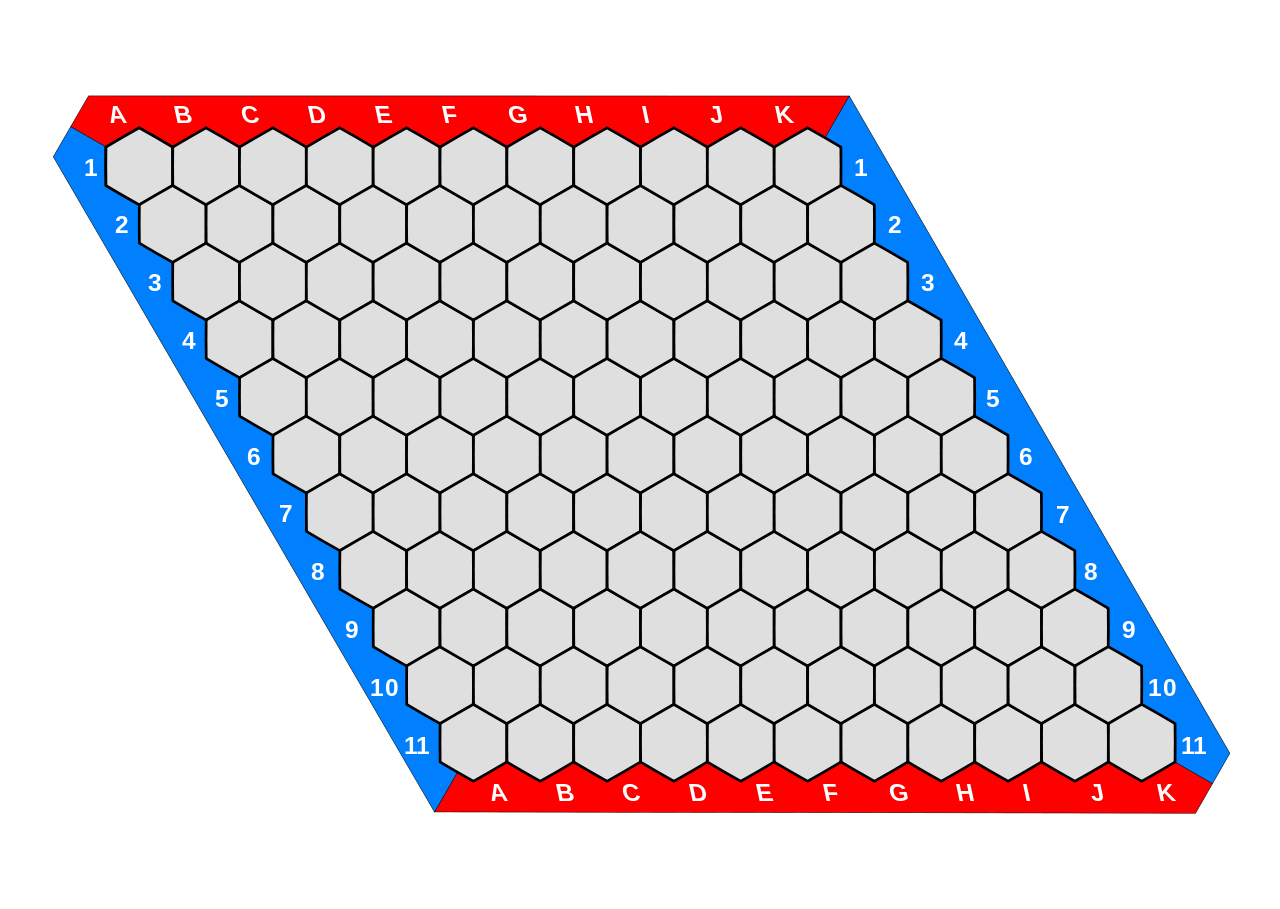
\includegraphics[scale=0.13]{11x11.png}
	\caption{Plateau de jeu 11x11}
\end{figure}

\subsection{Spécificités du jeu}

Une particularité du jeu de Hex est qu'il ne peut pas y avoir de partie aboutissant à un match nul. En effet, indépendamment des coups joués et de la taille du plateau, lorsque que le plateau est rempli, il y a obligatoirement un gagnant. Ce résultat a été établi par John Nash et repose sur une preuve par l'absurde \cite{hexwiki}.
Ainsi, pour des plateaux de tailles inférieures ou égales à 9x9, une stratégie gagnante \footnote{On appelle stratégie gagnante toute stratégie assurant la victoire quels que soient les choix que fait le joueur adverse.} est connue pour le premier joueur. Mais ce n'est pas le cas pour les plateaux de taille supérieure et des résultats de la théorie de la complexité montre que la recherche d'une telle stratégie devient très rapidement impraticable quand la taille du jeu augmente \footnote{Un plateau de taille classique, soit 11x11, a un facteur de branchement de 120.}. C'est pourquoi, nous allons adopter une approche statistique afin d'obtenir un comportement de jeu optimal de la part d'un joueur programmé avec des techniques d'intelligence artificielle.

\begin{figure}[h]
	\centering
	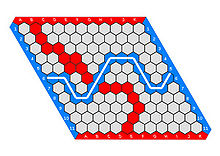
\includegraphics[scale=1]{11x11_gagnant.jpg}
	\caption{Configuration gagnante pour le joueur bleu}
\end{figure}

\section{Implémentation}

\subsection{Python Orienté Objet}

Le jeu a été implémenté en langage Python. Le module pygame a été utilisé pour l'interface graphique lorsque les parties se déroulent avec un joueur humain et le module multiprocessing a été utilisé pour augmenter la rapidité d'exécution des parties dans la phase de test des IA. Le projet est téléchargeable depuis \href{https://github.com/Maxime-LP/Hex-Game}{GitHub}.\\

Concernant la partie orienté objet, nous avons utilisé 3 classes. Une classe principale, \texttt{Game}, faisant interagir deux instances de la classe \texttt{Player} tour par tour en effectuant des actions sur l'objet de la classe \texttt{Board} représentant le plateau.

\subsection{Condition de fin de partie}

À chaque coup la fonction \texttt{check\_win} est appelée pour vérifier si la partie a été remportée par un joueur. La rapidité d'exécution de cette fonction a été la principale source d'amélioration qui nous a permis d'augmenter le nombre de parties simulées par seconde en jouant aléatoirement. Avec l'utilisation de multiprocessing, nous avons pu atteindre 23000 parties par seconde pour des parties sur des plateaux de taille 7x7 avec un ordinateur possédant un processeur muni de 48 cœurs.


\begin{figure}[h]
	\centering
	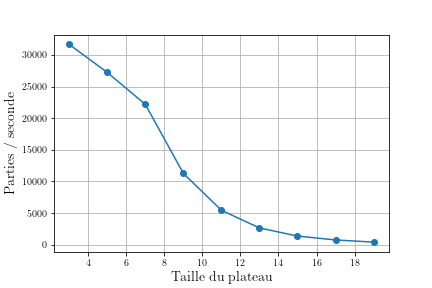
\includegraphics[scale=0.6]{pps.png}
	\caption{Rapidité d'exécution des parties}
	\label{fig:pps}
\end{figure}


Après une tentative avec la théorie des graphe et l'algorithme de Dijkstra, nous avons opté pour une méthode utilisant les composantes connexes par couleur du plateau. 
On considère qu'un joueur gagne s'il relie par une ligne continue les deux bords opposés du plateau, c'est-à-dire si les composantes connexes artificielles Nord et Sud ou Est et Ouest sont des sous-ensembles d'une même composante connexe.


Atteindre une bonne rapidité d'exécution en jouant aléatoirement est crucial car toutes les méthodes d'intelligence artificielle mises en œuvre par la suite en bénéficieront.

\newpage

\begin{lstlisting}
def check_win(self, currplayer):
	"""
	Checks if the current player won the game. 
	Returns the winner's name if there is any or None if there is none.
	1 : red player
	2 : blue player
	"""
	for component in self.board.components[currplayer.color - 1]:
		if currplayer.color == 1:
			if self.board.north_component.issubset(component) \
			and self.board.south_component.issubset(component):
				return currplayer
			
		else: 	# currplayer.color == 2
			if self.board.west_component.issubset(component) \
			and self.board.east_component.issubset(component):
				return currplayer
	return None
\end{lstlisting}

\newpage

\section{Joueur artificiel}

Au cours du projet, nous avons implémenté 4 algorithmes, chaque nouvelle version reprenant les bases de la précédente en y  ajoutant des améliorations. Le but étant que le joueur artificiel adopte des stratégies intelligentes en utilisant à son avantage la structure du plateau \footnote{On parle notamment ici des connections virtuelles et cases mortes (cf. p14).} sans programmer cela explicitement.

\subsection{Monte-Carlo}

\subsubsection{Principe}

La première méthode que nous avons programmé est une méthode naïve et empirique. Elle consiste simplement à simuler $n$ parties réparties équitablement entre les actions possibles pour déterminer le meilleur coup à jouer.

\subsubsection{Algorithme}

\begin{lstlisting}
def search(self, initialState):
	self.root = treeNode(initialState, None)
	actions = self.root.state.actions
	
	#On copie l'etat actuel du plateau
	for action in actions:
		root_state = deepcopy(self.root.state)
		root_state.takeAction(action, root_state.currplayer)
		node = treeNode(root_state, self.root)
		self.root.children[action] = node
		self.executeRound(node)
		
	#On simule un certain nombre de parties sur chaque action possible
	nb_iter = int(self.searchLimit / len(actions))
	for child in self.root.children.values():
		for i in range(nb_iter):
			self.executeRound(child)
		
	#On selectionne l'action menant au plus haut taux de victoire
	bestChild = self.getBestChild(self.root)
	action = (action for action, node in self.root.children.items() if node is bestChild).__next__()
		
	return action
\end{lstlisting}

Avec cette méthode et en simulant environ 10000 parties par coup disponible, il est possible de voir que le joueur artificiel commence à jouer des coups sensés. En effet, il joue majoritairement au centre du plateau, ce qui est une bonne stratégie puisque cela offre davantage de possibilités de connexions par la suite.

\newpage 


\subsection{Monte-Carlo et UCB1}

Le problème de l'algorithme Monte-Carlo naïf est qu'il utilise autant de simulations pour chaque coup. De ce fait, il utilise autant de ressources pour évaluer la qualité des mauvais coups que pour évaluer la qualité des bons coups. Le critère de sélection UCB1 permet de pallier ce problème.
Cet algorithme est nommé \texttt{mc\_ucb1} dans les fichiers Python.

\subsubsection{Principe}

Voici le fonctionnement de l'algorithme: 

\begin{figure}[h]
	\noindent\fbox{%
		\parbox{\textwidth}{%
			\textbf{UCB1} \\
			\textbf{Initialisation:} Jouer chaque coup une fois\\
			\textbf{Boucle:} Jouer le coup $j$ qui maximise $\bar{x_j} + c\sqrt{\frac{\ln{n}}{n_j} }$ avec $\bar{x_j}$ le taux de victoires du coup $j$ jusqu'à présent, $n_j$ le nombre de fois où le coup $j$ a été jouée, $n$ le nombre de coups total joués et $c$ une constante.     
		}%
	}
	\caption{Algorithme UCB1}
\end{figure}

Cet algorithme est initialement une réponse au problème du bandit manchot ou, dans sa version générale, du bandit à $K$ bras. Le problème original peut se formuler ainsi : un agent est face à des machines à sous dont il ne connaît pas les récompenses moyennes, son objectif est alors de maximiser ses gains.

Ce problème est en fait un exemple d'apprentissage par renforcement dans lequel l'agent doit faire des compromis entre l'exploitation de la machine qui empiriquement lui rapporte le plus et l'exploration des autres machines pour espérer trouver une machine rapportant davantage.

L'agent peut bien sûr adopter une approche naïve et jouer la machine maximisant la récompense moyenne sur les coups joués mais  cette stratégie peut le conduire à ignorer certaines machines, qui pourraient être plus intéressantes à jouer. \\

Peter Auer, Nicol\`o Cesa-Bianchi et Paul Fischer développent cette stratégie dans un article de référence, \textit{Finite-time Analysis of the Multiarmed Bandit Problem} \cite{ref1}, permettant à l'agent de continuer à explorer les machines tout en maximisant ses gains.\\

Le premier terme $\bar{x_j}$ représente la composante d'exploitation du critère UCB1 et le terme $\sqrt{\frac{\ln{n}}{n_j} }$ celui de l'exploration. La constante $c$ permet donc de donner plus ou moins d'importance à l'exploration. La constante théorique donnée dans le cadre du problème du bandit manchot est $c=\sqrt{2}$. Cependant, bien que des améliorations soient perceptibles par rapport à l'algorithme \texttt{mc} en utilisant cette constante, la constante d'exploration optimale n'est pas $\sqrt{2}$ dans notre cas. Nous reviendrons sur ce point dans la partie concernant l'algorithme UCT. \\

\newpage

\subsubsection{Algorithme}

Introduisons à présent les notions d'arbre et de nœud. On définit le nœud racine comme étant l'état initial du plateau de jeu, c'est le nœud parent. Ainsi, chaque nœud enfant représente un état du jeu avec 1 coup supplémentaire par rapport à son nœud parent. On lui affecte des attributs permettant de calculer son score avec le critère UCB1.

\begin{lstlisting}
	class treeNode():
	
		def __init__(self, state, parent):
			self.state = state
			self.parent = parent
			self.numVisits = 0
			self.totalReward = 0
			self.children = {}
			
			# self.root a la couleur du joueur adverse 
			# Les noeuds enfat sont de la couleur du joueur utilisant l'algorithme
			if parent is None : 
				self.player =  3 - state.player
			else:
				self.player = 3 - self.parent.player
\end{lstlisting}

Dans cet algorithme, l'arbre possède une profondeur de 1. La fonction retournant le meilleur coup pour l'algorithme \texttt{mc\_ucb1} est la suivante:

\begin{lstlisting}
def search(self, initialState):
	self.root = treeNode(initialState, None)
	actions = self.root.state.actions
	# Initialisation de chaque noeud
	...
	# Simulation avec selection des noeuds via UCB1
	for i in range(self.iterationLimit):
		child = self.ucb1(self.root, self.explorationConstant)
		self.executeRound(child)
		
	bestChild = self.ucb1(self.root, 0)
	action = (action for action, node in self.root.children.items() if node is bestChild).__next__()
	return action
	
def ucb1(self, node, explorationValue):
	bestValue = float("-inf")
	bestNodes = []
	for child in node.children.values():
		nodeValue = child.totalReward / child.numVisits + explorationValue * sqrt(log(node.numVisits) / child.numVisits )
		if nodeValue > bestValue:
			bestValue = nodeValue
			bestNodes = [child]
		elif nodeValue == bestValue:
			bestNodes.append(child)
	return random.choice(bestNodes)
\end{lstlisting}

La fonction \texttt{ucb1} calcule le score de chaque nœud via le critère UCB1. On note qu'une constante d'exploration nulle correspond au taux de parties gagnées pour un nœud.

\subsection{Upper Confidence Bound applied to Trees (UCT)}

L'algorithme \texttt{mc\_ucb1} permet d'optimiser les simulations sur un coup mais ne permet pas d'anticiper les états du jeu une fois ce coup joué. Il est alors intéressant d'effectuer une recherche arborescente du meilleur coup. Cette méthode est appelée Upper Confidence Bound applied to Trees, nommée \texttt{uct} dans les programmes Python. Cet algorithme de prise de décision est largement développé dans les jeux \footnote{On peut citer son utilisation dans certains programmes de Go, d'Échecs, de Shogi, ou encore le jeu Total War : Rome II}.

\subsubsection{Principe}

On initialise tous les nœuds de profondeur 1 en effectuant une simulation de parties aléatoires sur ces derniers avant de répéter les quatre étapes décrites ci-dessous. La figure 4 est prise comme exemple pour illustrer le propos.

\begin{figure}[h]
\centering
\includegraphics[scale=0.20]{étapes_mcts_.png}
\caption{Déroulement d'une simulation avec l'algorithme UCT}
\label{fig:uct}
\end{figure}

Précisons que le coup à la racine de l'arborescence est l'état actuel du plateau. De plus, les nœuds blancs correspondent à un coup joué par le joueur adverse.\\

1. Sélection\\
Premièrement, on effectue la phase de descente en sélectionnant les nœuds via le critère UCB1 jusqu'à atteindre un nœud sans enfant.\\
Exemple: Les nœuds gris sur la ligne de profondeur 1 ont pour score avec la constance théorique optimale $c=\sqrt{2}$ respectivement de la gauche à la droite $\frac{8}{10} + \sqrt{\frac{2\log21}{10}} \simeq 1,480$, $1.372$ et $1.425$. On choisit donc le nœud de gauche. Puis, on calcule de nouveau les scores des nœuds enfant, ici de profondeur 2. On obtient $1.573$ pour le nœud de gauche et $1.709$ pour le nœud de droite. On sélectionne donc le nœud de droite. Puis avec le même critère encore le nœud de droite de profondeur 3. On arrive à un nœud sans enfant aussi appelé feuille de l'arbre. C'est la fin de la première étape.
\\

2. Expansion\\
Deuxièmement, lorsqu'on atteint une feuille de l'arbre, on crée un nouveau nœud représentant un nouveau coup joué. Ce coup est choisi de manière aléatoire.\\

3. Simulation\\
Troisièmement, on finit la partie en sélectionnant les coups de manière aléatoire. Dans l'exemple la partie simulée a été perdue.\\

4. Rétro-propagation\\
Quatrièmement, on rétro-propage ce résultat jusqu'à la racine.\\
Exemple: On ajoute 1 au dénominateur (nombre de visites) pour chaque nœuds correspondant aux coups joués et on ajoute 1 au numérateur si la partie simulée a été gagnée et si le nœud est gris, c'est-à-dire si il correspond à un coup joué par le joueur artificiel ``utilisant'' l'algorithme.

Une fois les $n$ simulations effectuées, on sélectionne le nœud de profondeur 1 ayant le meilleur taux de victoire.

\subsubsection{Algorithme}

L'algorithme \texttt{uct} reprend en grande partie le code de l'algorithme \texttt{mc\_ucb1} mais avec une structure d'arbre.

\begin{lstlisting}
	def randomPolicy(state):
		while not state.isTerminal():
			action = random.choice(state.actions)
			state.takeAction(action, state.currplayer)
		return state.getReward()
	
	class treeNode():
		def __init__(self, state, parent):
			self.state = state
			self.parent = parent
			self.numVisits = 0
			self.totalReward = 0
			self.children = {}
			if parent is None : 
				self.player =  3 - state.player
			else:
				self.player = 3 - self.parent.player
	
	def isFullyExpanded(self):
		return len(self.state.actions)==len(self.children)
	
	class UCT():
		def __init__(self, explorationConstant,iterationLimit=None):
			self.iterationLimit = iterationLimit
			self.explorationConstant = explorationConstant
			self.rollout = randomPolicy
		
		def search(self, initialState):
			self.root = treeNode(initialState, None) if root==None else root
			for i in range(self.iterationLimit):
				self.executeRound()
			bestChild = self.getBestChild(self.root, 0)
			action = (action for action, node in self.root.children.items() if node is bestChild).__next__()
			return action
		
		def executeRound(self):
			node = self.selectNode(self.root)
			state = deepcopy(node.state)
			reward = self.rollout(state)
			self.backpropogate(node, reward)
		
		def selectNode(self, node):
			while not node.state.isTerminal():
				if node.isFullyExpanded():
					node = self.getBestChild(node, self.explorationConstant)
				else:
					return self.expand(node)
			return node
		
		def expand(self, node):
			actions = node.state.getPossibleActions()
			while actions!=[]:
				action = random.choice(actions)
				if action not in node.children.keys():
					node_state = deepcopy(node.state)
					node_state.takeAction(action, node_state.currplayer)
					newNode = treeNode(node_state, node)
					node.children[action] = newNode
					return newNode
			
		def backpropogate(self, node, reward):
			while node is not None:
				node.numVisits += 1
				node.totalReward += (reward == 1) * (node.player != self.root.player)
				node = node.parent
		
		def getBestChild(self, node, explorationValue):
			return self.ucb1(node,explorationValue)
		
		def ucb1(self,node,explorationValue):
			bestValue = float("-inf")
			bestNodes = []
			for child in node.children.values():
				nodeValue = child.totalReward / child.numVisits + explorationValue * sqrt(log(node.numVisits) / child.numVisits)
				if nodeValue > bestValue:
					bestValue = nodeValue
					bestNodes = [child]
				elif nodeValue == bestValue:
					bestNodes.append(child)
			return random.choice(bestNodes)
\end{lstlisting}

\newpage

\subsubsection{Constante d'exploration optimale}

La constante d'exploration optimale ne correspond pas à la valeur théorique $c=\sqrt{2}$. En pratique, cette dernière est plus faible pour le jeu de Hex que pour le problème des bandits manchots. Les meilleurs résultats sont obtenus pour $c \simeq 0.3$. Cette observation empirique est partagée pour les jeux ayant des récompenses entre 0 et 1 \cite{expcst}, ce qui est le cas ici : une partie gagnée vaut une récompense de 1 et une partie perdue donne une récompense nulle.

\begin{figure}[!h]
	\centering
	\begin{subfigure}{0.49\textwidth}
		\centering
		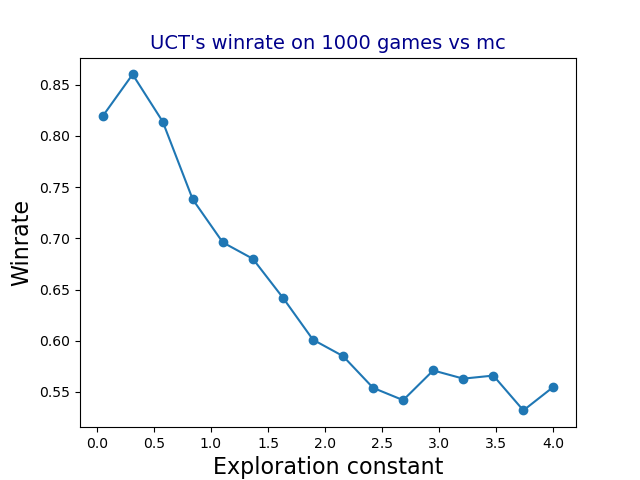
\includegraphics[width=\textwidth]{test1.png}
		\caption{contre \texttt{mc}}
		\label{fig:1_}
	\end{subfigure}
	\hfill
	\begin{subfigure}{0.49\textwidth}
		\centering
		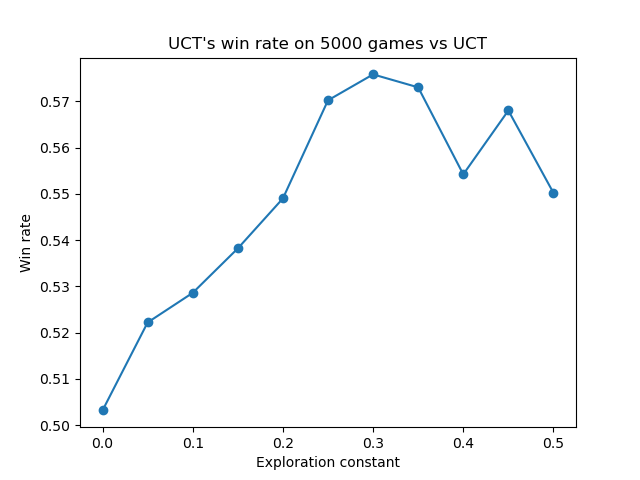
\includegraphics[width=\textwidth]{test2.png}
		\caption{contre \texttt{uct} avec $c = \sqrt{2}$}
		\label{fig:2_}
	\end{subfigure}
	\hfill
	\begin{subfigure}{0.5\textwidth}
		\centering
		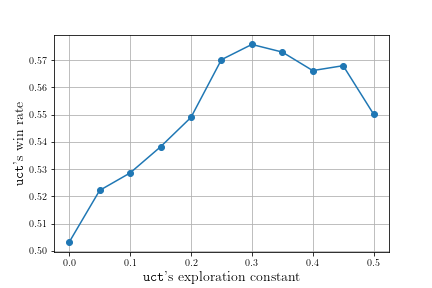
\includegraphics[width=\textwidth]{test3.png}
		\caption{contre \texttt{uct} avec $c = \sqrt{2}$}
		\label{fig:3_}
	\end{subfigure}
	\caption{Constante d'exploration optimale pour UCT avec $n=100$}
	\label{fig:best-cst}
\end{figure}

\subsection{UCT avec mémoire}

Pour aller plus loin, l'algorithme \texttt{uct} pourrait garder en mémoire une partie de l'arbre pour ses coups suivants. En effet, après avoir joué une première fois, le joueur artificiel \texttt{uct} pourrait tronquer l'arbre et considérer comme racine le nœud correspondant à l'état actuel du plateau, ce qui lui permettrait de conserver les simulations déjà effectuées.\\
Nous prenons comme exemple la figure 7. Si on considère que \texttt{uct} a joué le coup bleu puis son adversaire le coup rouge,  et que le nœud rouge a été visité précédemment, alors on récupère comme racine le nœud rouge avec ses enfants.\\

\begin{figure}[h]
	\centering
	\includegraphics[scale=0.5]{arbre_tronqué.png}
	\caption{Arbre tronqué}
	\label{fig:arbre-tronqué}
\end{figure}

\newpage

Cependant cette méthode ne produit pas d'amélioration significative si le nombre de simulations par coup n'est pas assez grand.

\newpage

\section{Évaluation des algorithmes}

Pour évaluer les performances des algorithmes nous les avons fait jouer sur un plateau 7x7 avec comme témoin l'algorithme \texttt{uct}. Ces comparaisons ont été faites pour 100, 1000 et 10000 parties simulées à chaque fois ainsi que pour \texttt{uct} en premier et deuxième joueur.

\begin{figure}[!h]
	\centering
	\begin{subfigure}{0.49\textwidth}
		\centering
		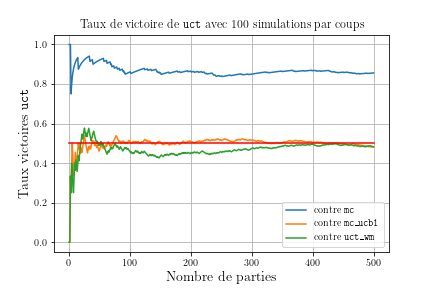
\includegraphics[width=\textwidth]{n100_uct_snd.png}
		\caption{\texttt{uct} premier joueur}
		\label{fig:n100-uct-snd}
	\end{subfigure}
	\hfill
	\begin{subfigure}{0.49\textwidth}
		\centering
		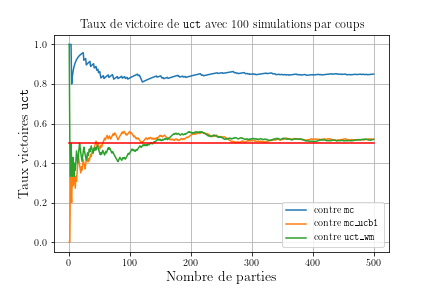
\includegraphics[width=\textwidth]{n100_uct_first.png}
		\caption{\texttt{uct} second joueur}
		\label{fig:n100-uct-first}
	\end{subfigure}
	\caption{100 parties simulées par coups}
	\label{fig:n100}
\end{figure}

\begin{figure}[!h]
	\centering
	\begin{subfigure}{0.49\textwidth}
		\centering
		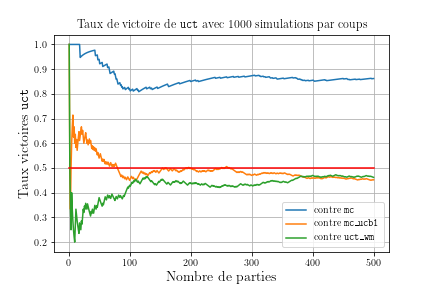
\includegraphics[width=\textwidth]{n1000_uct_snd.png}
		\caption{\texttt{uct} premier joueur}
		\label{fig:n1000-uct-snd}
	\end{subfigure}
	\hfill
	\begin{subfigure}{0.49\textwidth}
		\centering
		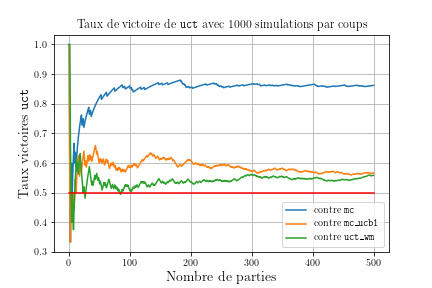
\includegraphics[width=\textwidth]{n1000_uct_first.png}
		\caption{\texttt{uct} second joueur}
		\label{fig:n1000-uct-first}
	\end{subfigure}
	\caption{1000 parties simulées par coups}
	\label{fig:n1000}
\end{figure}

\begin{figure}[!h]
	\centering
	\begin{subfigure}{0.49\textwidth}
		\centering
		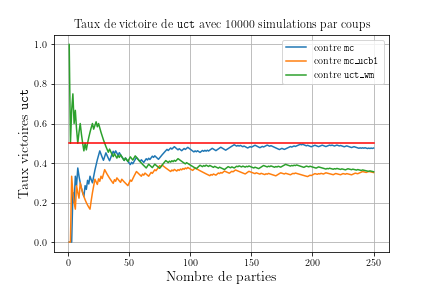
\includegraphics[width=\textwidth]{n10000_uct_snd.png}
		\caption{\texttt{uct} premier joueur}
		\label{fig:n10000-uct-snd}
	\end{subfigure}
	\hfill
	\begin{subfigure}{0.49\textwidth}
		\centering
		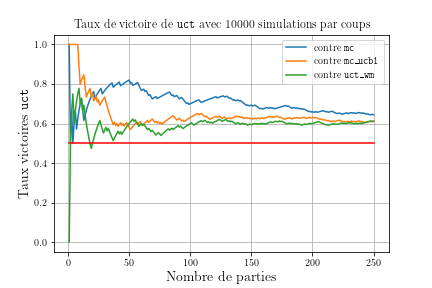
\includegraphics[width=\textwidth]{n10000_uct_first.png}
		\caption{\texttt{uct} second joueur}
		\label{fig:n10000-uct-first}
	\end{subfigure}
	\caption{10000 parties simulées par coups}
	\label{fig:n10000}
\end{figure}

\newpage

\section{Axes d'amélioration}

\subsection{Multiprocessing}

Au cours de l'algorithme UCT, la puissance de calcul est utilisée par deux tâches en particulier : se déplacer dans l'arbre et effectuer des simulations aléatoires. La partie simulation aléatoire est celle qui prend la majorité du temps de calcul. Une structure que l'on appelle maître/esclave peut améliorer la rapidité de l'algorithme. Le maître effectue les déplacements au sein de l'arbre puis les processus esclaves effectuent les simulations pour finir les parties. Un gain de rapidité pourrait être envisagé en augmentant le nombre de parties par coup et en faisant une dizaine, voir plus, de simulations à chaque nœud enfant.

\subsection{Début de partie}

Un autre axe d'amélioration se trouve en début de partie. Plus il y a de coups possibles, moins les estimations de la qualité de ces derniers sont justes. C'est pourquoi compléter l'algorithme \texttt{uct} avec une autre approche serait intéressant. Il existe pour cela les algorithmes RAVE et GRAVE \cite{rave} \cite{grave}.

\newpage

\section{Conclusion}

Les résultats montrent une grande amélioration des performances grâce à l'utilisation du critère UCB1 permettant de simuler moins de parties sur les coups jugés mauvais. Cette différence se réduit à mesure que le nombre de parties simulées par coup augmente. De plus, on observe que commencer à jouer en premier donne un avantage de plus en plus significatif lorsque ce dernier augmente.
Enfin l'algorithme UCT permet d'obtenir de bons résultats avec des capacités de calculs relativement faibles. En effet, à partir de plusieurs milliers de simulations par coup, soit moins de 5 secondes de calcul sur un ordinateur lambda, il est possible de voir que l'algorithme tire partie des propriétés géométriques du jeu. Parmi ces propriétés, nous pouvons citer les connexions virtuelles , les cases mortes ou encore les échelles. Faire intégrer ces notions à UCT pourrait être une ultime piste d'amélioration.

\newpage

\listoffigures 

\newpage

\nocite{ref2}
\bibliographystyle{plain}
\bibliography{biblio}

\end{document}